\subsubsection{Characteristic faults}
\label{desc_characteristic_fault}
\index{Source type!fault!characteristic}
\index{Characteristic fault|see{Source type}}

The characteristic fault source is a particular typology of fault created
with the assumption that its ruptures will always cover the entire fault
surface. As such, no floating is necessary on the surface. The characteristic fault may still take as input a magnitude frequency distribution. In this case, the fault surface can be represented either as a \gls{simplefaultsource} surface or as a \gls{complexfaultsource} surface or as a combination of rectangular ruptures as represented in
Figure~\ref{fig:char_fault_source}. Mutiple surfaces containing mixed geometry types are also supported. 

\begin{figure}[htb]
\centering
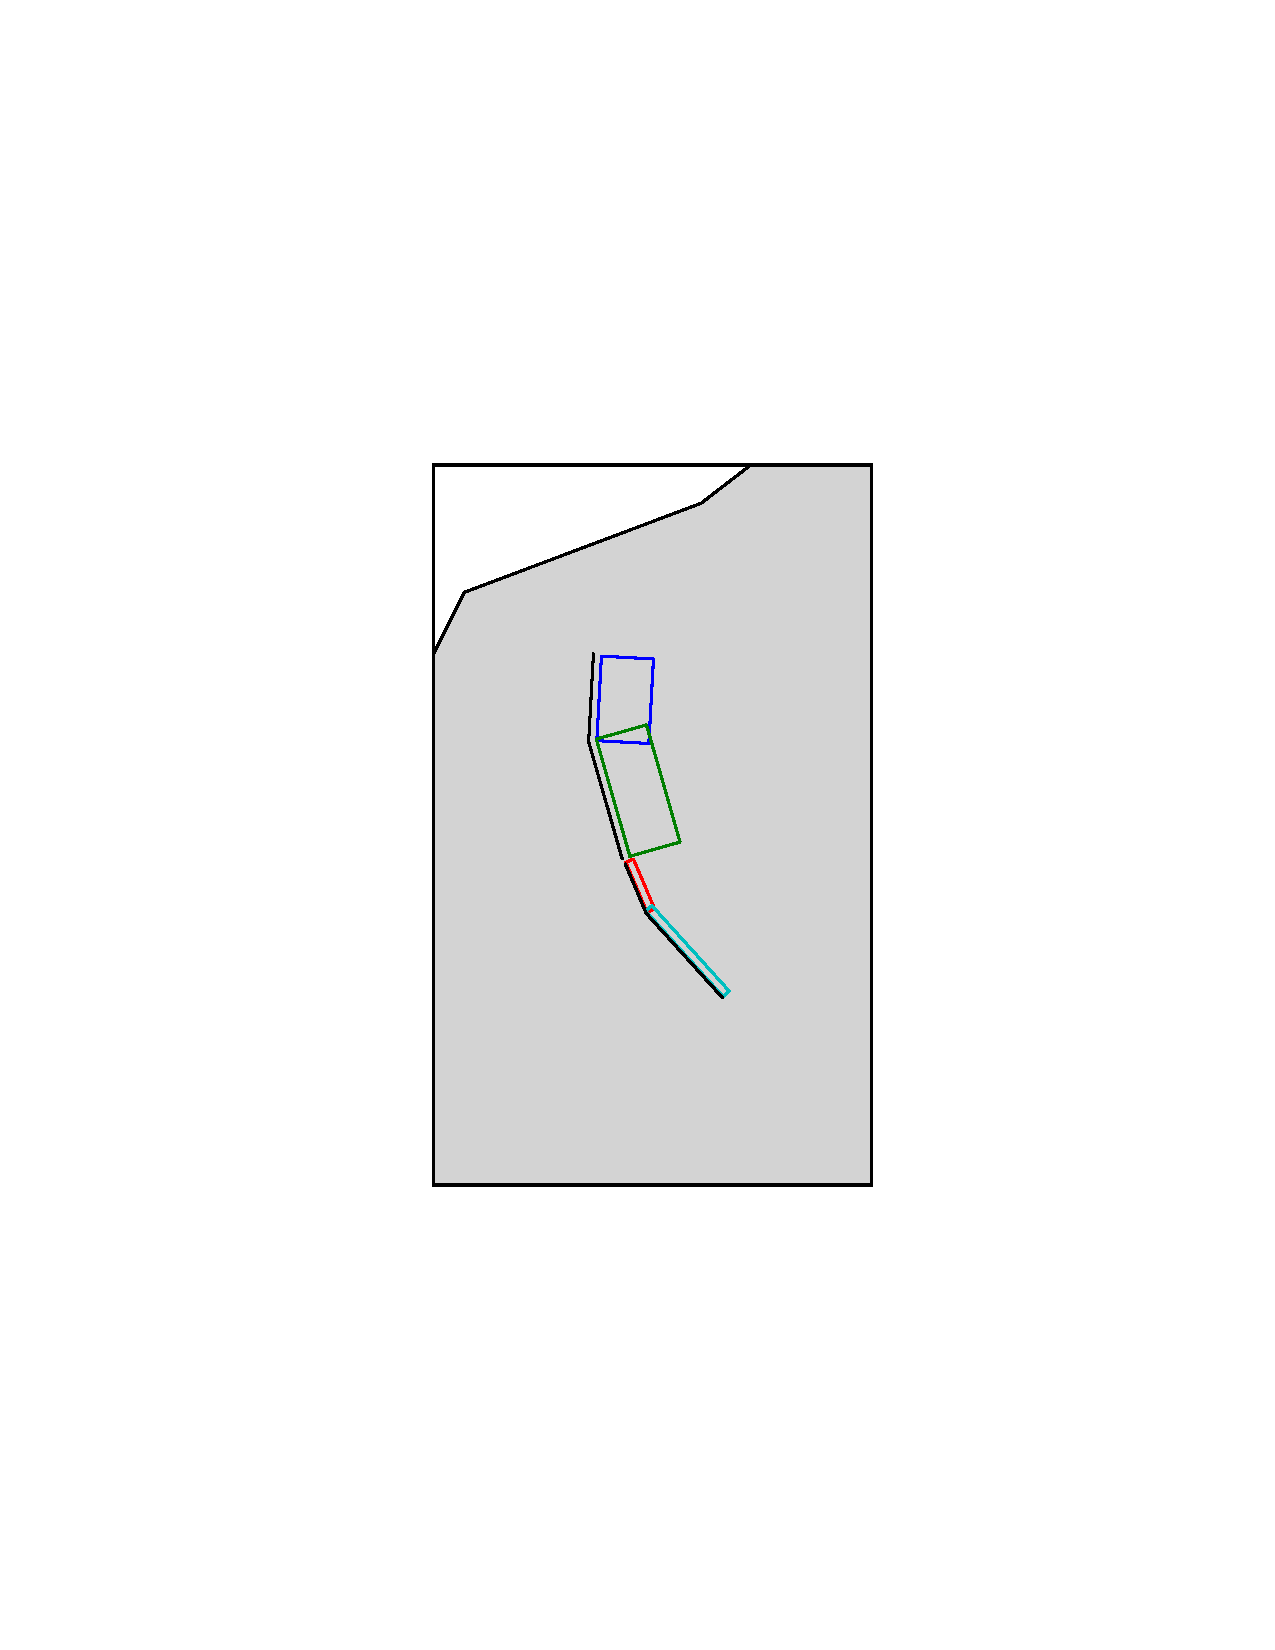
\includegraphics[trim=5cm 7cm 5cm 7cm, clip, width=10cm]{figures/hazard/multi_surface.pdf}
\caption{Geometry of a multi-segmented characteristic fault composed of four
         rectangular ruptures as modelled in OpenQuake.}
\label{fig:char_fault_source}
\end{figure}

\paragraph{Source data}
\begin{itemize}
    \item The characteristic rupture surface is defined through one of the
    following options:
        \begin{itemize}
            \item A list of rectangular ruptures (``planar surfaces'')
            \item A \gls{simplefaultsource} geometry
            \item A \gls{complexfaultsource} geometry
        \end{itemize}
    \item A \gls{frequencymagnitudedistribution}.
    \item Rake angle (specified following the Aki-Richards convention; see
          \citet{aki2002}).
    \item Upper and lower depth values limiting the seismogenic interval.
\end{itemize}

A comprehensive example enumerating the possible rupture surface configurations is shown below. 

\inputminted[firstline=1,firstnumber=1,fontsize=\footnotesize,frame=single,linenos,bgcolor=lightgray]{xml}{oqum/hazard/verbatim/input_characteristic_fault_simple.xml}
\captionof{listing}{Example characteristic fault with simple fault geometry\label{lst:example_characteristic_fault_simple}}

\inputminted[firstline=1,firstnumber=1,fontsize=\footnotesize,frame=single,linenos,bgcolor=lightgray]{xml}{oqum/hazard/verbatim/input_characteristic_fault_complex.xml}
\captionof{listing}{Example characteristic fault with complex fault geometry\label{lst:example_characteristic_fault_complex}}

\inputminted[firstline=1,firstnumber=1,fontsize=\footnotesize,frame=single,linenos,bgcolor=lightgray]{xml}{oqum/hazard/verbatim/input_characteristic_fault_planar.xml}
\captionof{listing}{Example characteristic fault with planar/multi-planar fault geometry\label{lst:example_characteristic_fault_planar}}



%\begin{mdframed}[]
%\inputminted[firstline=1,firstnumber=1,fontsize=%\footnotesize,frame=single,linenos,bgcolor=lightgray]{xml}{oqum/hazard/verbatim/input_nonparametric_source.xml}
%\caption{Example non-parametric source with planar, multi-planar, simple fault %and complex fault geometry}
%\label{lst:example_nonparametric_source}
%\end{mdframed}
%\begin{Verbatim}[frame=single, commandchars=\\\{\}, fontsize=\footnotesize,
    numbers=left, numbersep=2pt]
<?xml version="1.0" encoding="utf-8"?>
<nrml
xmlns="http://openquake.org/xmlns/nrml/0.5"
xmlns:gml="http://www.opengis.net/gml"
>
    <sourceModel name="Test Source Model">
        <nonParametricSeismicSource id="1"
        name="A Non Parametric Source" tectonicRegion="Some TRT">
            <singlePlaneRupture probs_occur="0.544 0.456">
\textcolor{blue}{               <magnitude>8.3</magnitude>}
\textcolor{blue}{               <rake>90.0</rake>}
\textcolor{red}{               <hypocenter depth="26.101" lat="40.726" lon="143.0"/>}
\textcolor{red}{               <planarSurface>}
\textcolor{red}{                   <topLeft depth="9.0" lat="41.6" lon="143.1"/>}
\textcolor{red}{                   <topRight depth="9.0" lat="40.2" lon="143.91"/>}
\textcolor{red}{                   <bottomLeft depth="43.202" lat="41.252" lon="142.07"/>}
\textcolor{red}{                   <bottomRight depth="43.202" lat="39.852" lon="142.91"/>}
\textcolor{red}{               </planarSurface>}
           </singlePlaneRupture>
          <multiPlanesRupture probs_occur="0.9244 0.0756">
\textcolor{blue}{               <magnitude>6.9</magnitude>}
\textcolor{blue}{               <rake>0.0</rake>}
\textcolor{red}{               <hypocenter depth="7.1423" lat="35.296" lon="139.31"/>}
\textcolor{red}{               <planarSurface>}
\textcolor{red}{                   <topLeft depth="2.0" lat="35.363" lon="139.16"/>}
\textcolor{red}{                   <topRight depth="2.0" lat="35.394" lon="138.99"/>}
\textcolor{red}{                   <bottomLeft depth="14.728" lat="35.475" lon="139.19"/>}
\textcolor{red}{                   <bottomRight depth="14.728" lat="35.505" lon="139.02"/>}
\textcolor{red}{               </planarSurface>}
\textcolor{red}{               <planarSurface>}
\textcolor{red}{                   <topLeft depth="2.0" lat="35.169" lon="139.34"/>}
\textcolor{red}{                   <topRight depth="2.0" lat="35.358" lon="139.17"/>}
\textcolor{red}{                   <bottomLeft depth="12.285" lat="35.234" lon="139.45"/>}
\textcolor{red}{                   <bottomRight depth="12.285" lat="35.423" lon="139.28"/>}
\textcolor{red}{               </planarSurface>}
           </multiPlanesRupture>
           <simpleFaultRupture probs_occur="0.157 0.843">
\textcolor{blue}{               <magnitude>7.8</magnitude>}
\textcolor{blue}{               <rake>90.0</rake>}
\textcolor{red}{               <hypocenter depth="22.341" lat="43.624" lon="147.94"/>}
\textcolor{red}{               <simpleFaultGeometry>}
\textcolor{red}{                   <gml:LineString>}
\textcolor{red}{                       <gml:posList>}
\textcolor{red}{                           147.96 43.202}
\textcolor{red}{                           148.38 43.438}
\textcolor{red}{                           148.51 43.507}
\textcolor{red}{                           148.68 43.603}
\textcolor{red}{                           148.76 43.640}
\textcolor{red}{                       </gml:posList>}
\textcolor{red}{                   </gml:LineString>}
\textcolor{red}{                   <dip>30.0</dip>}
\textcolor{red}{                   <upperSeismoDepth>14.5</upperSeismoDepth>}
\textcolor{red}{                   <lowerSeismoDepth>35.5</lowerSeismoDepth>}
\textcolor{red}{               </simpleFaultGeometry>}
           </simpleFaultRupture>
           <complexFaultRupture probs_occur="0.157 0.843">
\textcolor{blue}{               <magnitude>7.8</magnitude>}
\textcolor{blue}{               <rake>90.0</rake>}
\textcolor{red}{               <hypocenter depth="22.341" lat="43.624" lon="147.94"/>}
\textcolor{red}{               <complexFaultGeometry>}
\textcolor{red}{                   <faultTopEdge>}
\textcolor{red}{                       <gml:LineString>}
\textcolor{red}{                           <gml:posList>}
\textcolor{red}{                               148.76 43.64 5.0}
\textcolor{red}{                               148.68 43.603 5.0}
\textcolor{red}{                               148.51 43.507 5.0}
\textcolor{red}{                               148.38 43.438 5.0}
\textcolor{red}{                               147.96 43.202 5.0}
\textcolor{red}{                           </gml:posList>}
\textcolor{red}{                       </gml:LineString>}
\textcolor{red}{                   </faultTopEdge>}
\textcolor{red}{                   <faultBottomEdge>}
\textcolor{red}{                      <gml:LineString>}
\textcolor{red}{                           <gml:posList>}
\textcolor{red}{                               147.92 44.002 35.5}
\textcolor{red}{                               147.81 43.946 35.5}
\textcolor{red}{                               147.71 43.897 35.5}
\textcolor{red}{                               147.5 43.803 35.5}
\textcolor{red}{                               147.36 43.727 35.5}
\textcolor{red}{                           </gml:posList>}
\textcolor{red}{                       </gml:LineString>}
\textcolor{red}{                   </faultBottomEdge>}
\textcolor{red}{               </complexFaultGeometry>}
            </complexFaultRupture>
        </nonParametricSeismicSource>
    </sourceModel>
</nrml>
\end{Verbatim}


